\section{Korrelationsmatrizen sortiert nach Gemeindeschlüssel}
\subsection{Korrelationsmatrizen mit den nach Gemeindeschlüsseln sortierten Landkreisen}\label{sec:Durchführung:Korrelationsmatrizen mit den nach Gemeindeschlüsseln sortierten Landkreisen}
In \autoref{fig:matrizes_north_to_south_counties} befinden sich die vier Matrizen mit den Werten für die Korrelationen zwischen den Landkreisen.
Die Zeilen und Spalten sind lexikographisch nach den Gemeindeschlüsseln der Landkreise sortiert und diesen zugeordnet. In \autoref{tab:counties_by_admunitid} befindet sich die komplette sortierte Liste der Landkreise.

In den Matrizen zeichnet sich bereits eine auffällige Einteilung ab: Die Spalten im linken Drittel scheinen eher niedrige Werte zu enthalten, wohingegen die restlichen Spalten eher durchmischt sind jedoch im Vergleich zu den Spalten im linken Drittel eher hohe Werte enthalten.
\begin{figure}[H]
    \centering
    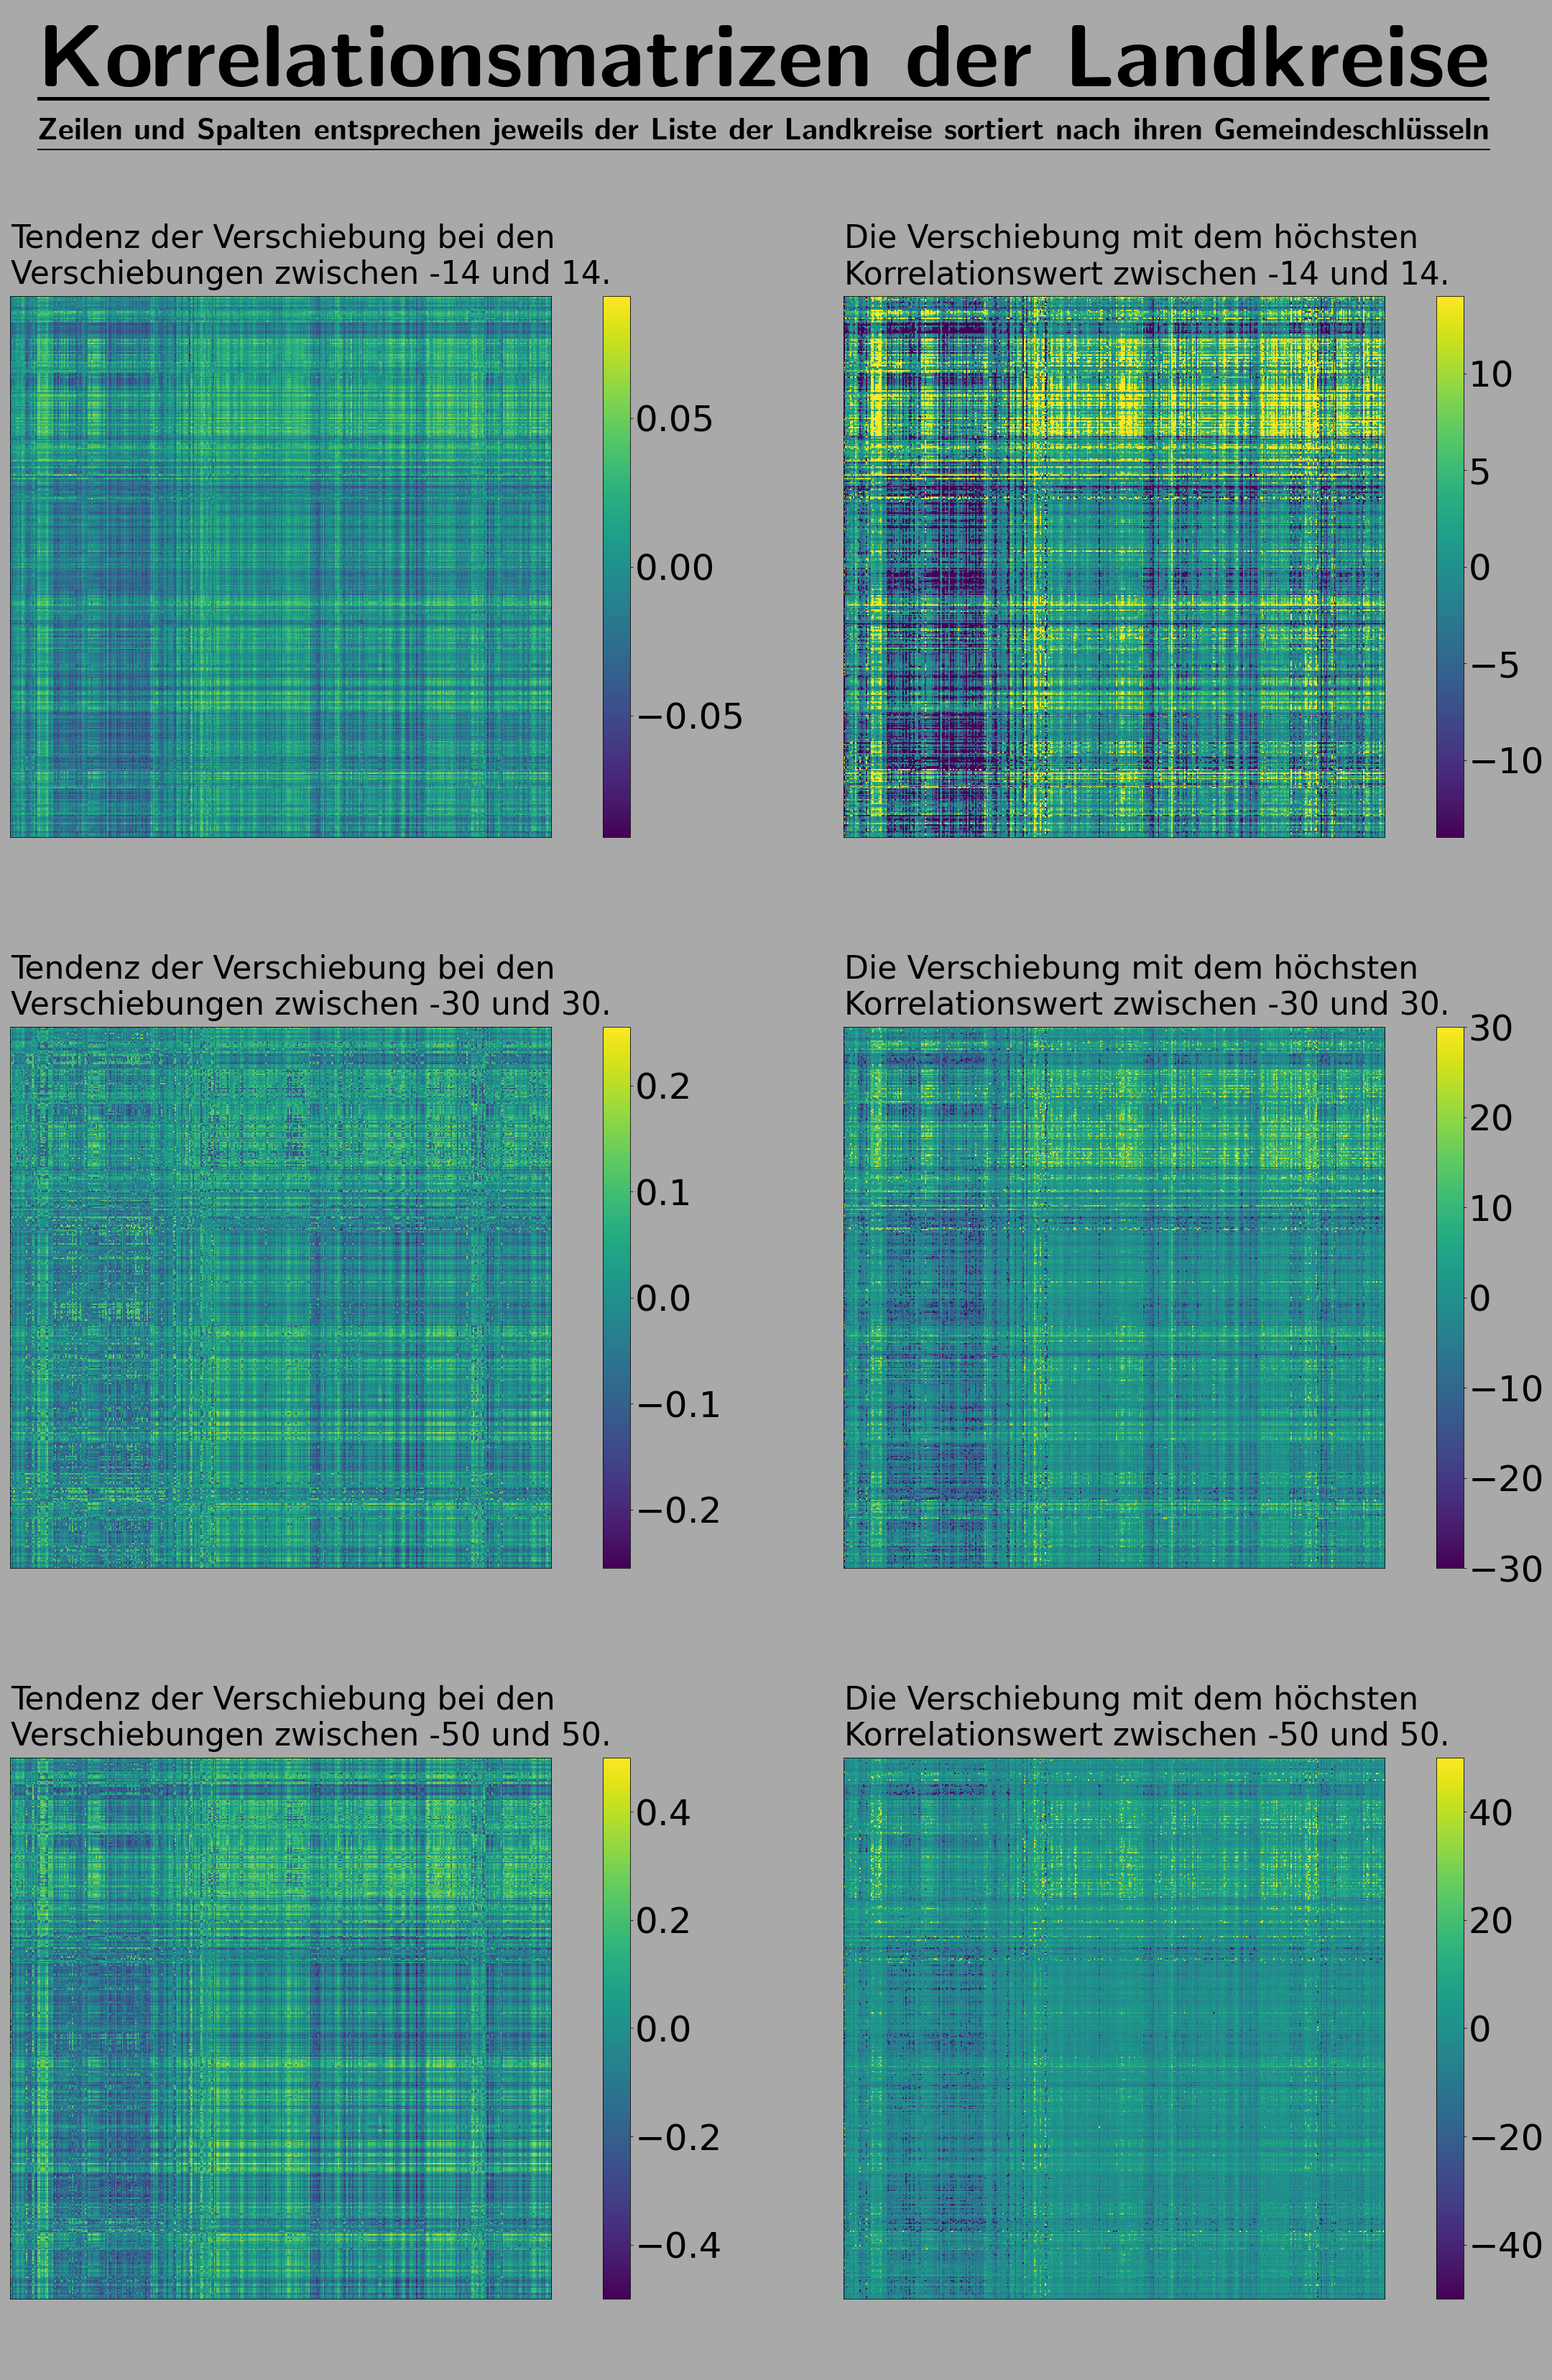
\includegraphics[width = 0.95\textwidth]{figures/Ergebnisse/matrizes_north_to_south_counties.png}
    \caption{Korrelationsmatrizen der Korrelationen aller Landkreise lexikographisch sortiert (siehe \autoref{tab:counties_by_admunitid}). Die Farben der Zellen der oberen Matrizen entsprechen den Tendenzen der Verschiebung $\hat{\tau}$ des Landkreises der Spalte in Relation zum Landkreis der Zeile nach \autoref{eq:Tendenz der Verschiebung}. 
    In den unteren Matrizen wird die Zelle entsprechend der Verschiebung $\tau_0$ der Zeitreihe des Landkreises der Spalte entgegen der Zeitreihe der Zeile mit dem höchsten Korrelationswert $c(\tau_0)$ eingefärbt. Links sind die Kennzahlen aus den Verschiebungen $\tau\in[-14,14]$ und rechts aus den Verschiebungen $\tau\in[-30,30]$ ausgewählt und berechnet worden.
    }
    \label{fig:matrizes_north_to_south_counties}
\end{figure}
\subsection{Korrelationsmatrizen mit den nach Gemeindeschlüsseln sortierten Regierungsbezirken}\label{sec:Durchführung:Korrelationsmatrizen mit den nach Gemeindeschlüsseln sortierten Regierungsbezirken}

Die vier Matrizen mit den Werten für die Korrelationen zwischen den Regierungsbezirken befinden sich in \autoref{fig:matrizes_north_to_south_districts}. Auch hier sind die Zeilen und Spalten lexikographisch nach den Gemeindeschlüsseln der Landkreise in den Regierungsbezirken sortiert. Die vollständige Auflistung von diesen befindet sich im Anhang in \autoref{tab:districts_by_admunitid}.

Die in \autoref{sec:Durchführung:Korrelationsmatrizen mit den nach Gemeindeschlüsseln sortierten Landkreisen} beschriebene Aufteilung findet sich auch in diesen Matrizen: Die Spalten im linken Drittel besitzen bis auf die dritte und elfte Spalte eher negative Werte und die Spalten in den anderen beiden Dritteln sind eher positiv. Aus der Auflistung der Regierungsbezirke in \autoref{tab:districts_by_admunitid} ergibt sich, dass die dritte und elfte Spalte den beiden Stadtstaaten Berlin und Hamburg zugeordnet sind.

\begin{figure}[H]
    \centering
    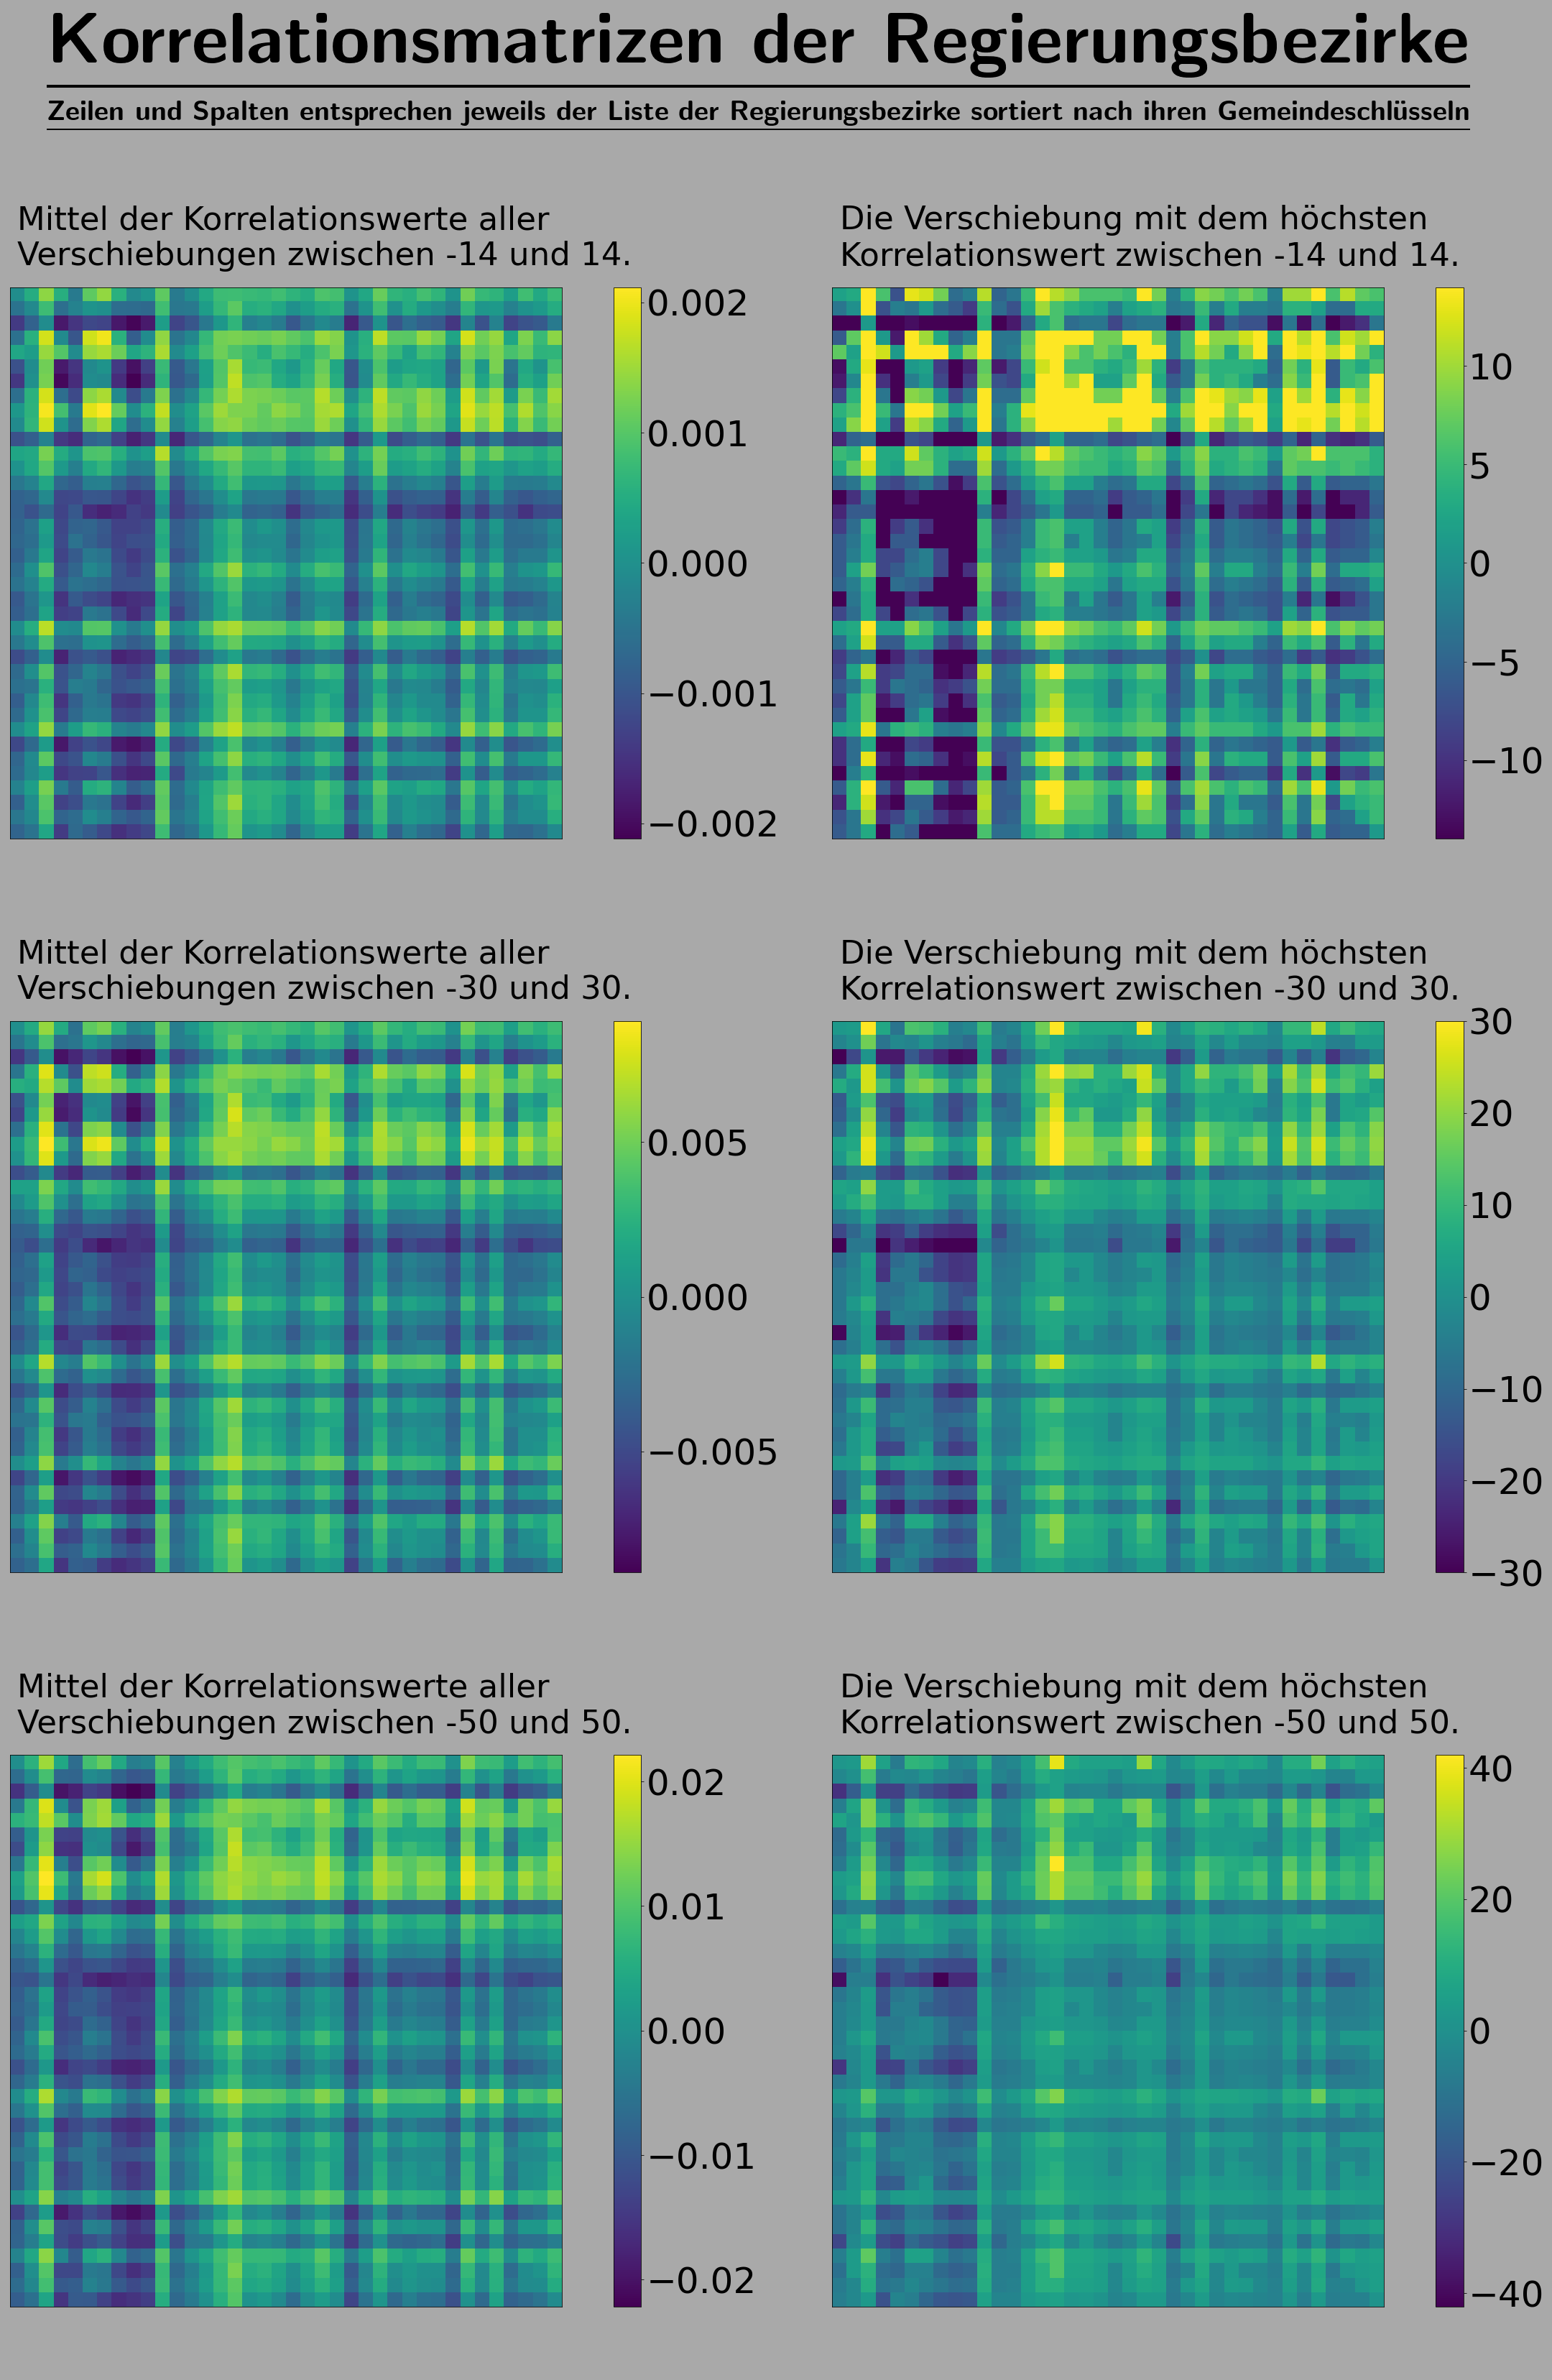
\includegraphics[width = 0.95\textwidth]{figures/Ergebnisse/matrizes_north_to_south_districts.png}
    \caption{Korrelationsmatrizen der Korrelationen aller Regierungsbezirke lexikographisch sortiert (siehe \autoref{tab:districts_by_admunitid}). Die Farben der Zellen der oberen Matrizen entsprechen den Tendenzen der Verschiebung $\hat{\tau}$ des Regierungsbezirks der Spalte in Relation zum Regierungsbezirk der Zeile nach \autoref{eq:Tendenz der Verschiebung}. 
    In den unteren Matrizen wird die Zelle entsprechend der Verschiebung $\tau_0$ der Zeitreihe des Regierungsbezirks der Spalte entgegen der Zeitreihe der Zeile mit dem höchsten Korrelationswert $c(\tau_0)$ eingefärbt. Links sind die Kennzahlen aus den Verschiebungen $\tau\in[-14,14]$ und rechts aus den Verschiebungen $\tau\in[-30,30]$ ausgewählt und berechnet worden.
    }
    \label{fig:matrizes_north_to_south_districts}
\end{figure}